% Created 2020-08-21 Fri 14:46
% Intended LaTeX compiler: pdflatex
\documentclass[a4paper,11pt]{article}
\usepackage[utf8]{inputenc}
\usepackage[T1]{fontenc}
\usepackage{graphicx}
\usepackage{grffile}
\usepackage{longtable}
\usepackage{wrapfig}
\usepackage{rotating}
\usepackage[normalem]{ulem}
\usepackage{amsmath}
\usepackage{textcomp}
\usepackage{amssymb}
\usepackage{capt-of}
\usepackage{hyperref}
\usepackage{rotating}
\usepackage{pdflscape}
\author{Tigany Zarrouk}
\date{\today}
\title{Atomistic investigation of dislocation-assisted carbon migration in iron}
\hypersetup{
 pdfauthor={Tigany Zarrouk},
 pdftitle={Atomistic investigation of dislocation-assisted carbon migration in iron},
 pdfkeywords={},
 pdfsubject={},
 pdfcreator={Emacs 26.3 (Org mode 9.1.9)}, 
 pdflang={English}}
\begin{document}

\maketitle
\tableofcontents

\clearpage

\begin{abstract}
Martensitic bearing steels have been shown to undergo subsurface microstructural decay, forming
Dark Etching Regions (DERs), promoting failure through rolling contact fatigue
(RCF). Dislocation-assisted carbon migration is thought to be the underlying mechanism, yet
empirical studies have been inconclusive as to how dislocations move carbon and where excess
carbon from the martensitic matrix migrates to upon transformation to ferrite---a phase of
significantly lower carbon solubility. In this report, we detail the first stage of a multi-scale
modelling approach to elucidate carbon transport by dislocations. Tight-binding simulations of
carbon interactions with the $1/2\langle 111 \rangle$ screw dislocation found solute distribution to vary
significantly within $\sim2$b of the easy and hard cores; the highest binding energy being found in
the centre of the hard screw core---which is the ground state carbon-dislocation
configuration---in agreement with Density Functional Theory (DFT). Determination of equilibrium
carbon concentration along dislocation lines, at various dislocation densities and nominal carbon
concentrations, found most sites around the hard core were saturated, with all easy cores
reconstructing to hard due to saturation of adjacent octahedral sites. In the typical temperature
range of bearing operation, we expect all dislocations to be of hard core type, pinned by carbon
in a prismatic site within the dislocation core. We anticipate large drag forces acting on
dislocations in the initial stages of glide, due to carbon-dislocation binding. These atomistic
results provide data for the last two stages in this multi-scale approach: determination
of kink-pair formation energies as a function of stress and carbon concentration using a line
tension model of a dislocation, and kinetic Monte Carlo (kMC) simulations incorporating solute
diffusion, to ascertain how carbon moves with dislocations in different stress, temperature and
concentration regimes.

\end{abstract}

\clearpage

\section{Introduction}
\label{sec:org8d51cc7}

Martensitic steels are frequently used in bearings due to their resilience to service conditions,
being subject to high rotational speeds and contact pressures. However, under cyclic loading
exceeding a given contact stress, the microstructure of the steel can decay due to the accumulation
of plasticity. This signals the onset of rolling cycle fatigue (RCF), which increases the risk of
failure from subsurface crack initiation. The microstructural decay corresponds to the observation
of Dark Etching Regions (DERs) as seen in optical microscopy, where the darkness of these regions is due
to the higher reactivity of DER phases to the etchant; exacerbated by
the roughness of the DER region \cite{skf2019}. See figure \ref{fuderpicture}.

\begin{figure}[htbp]
\centering
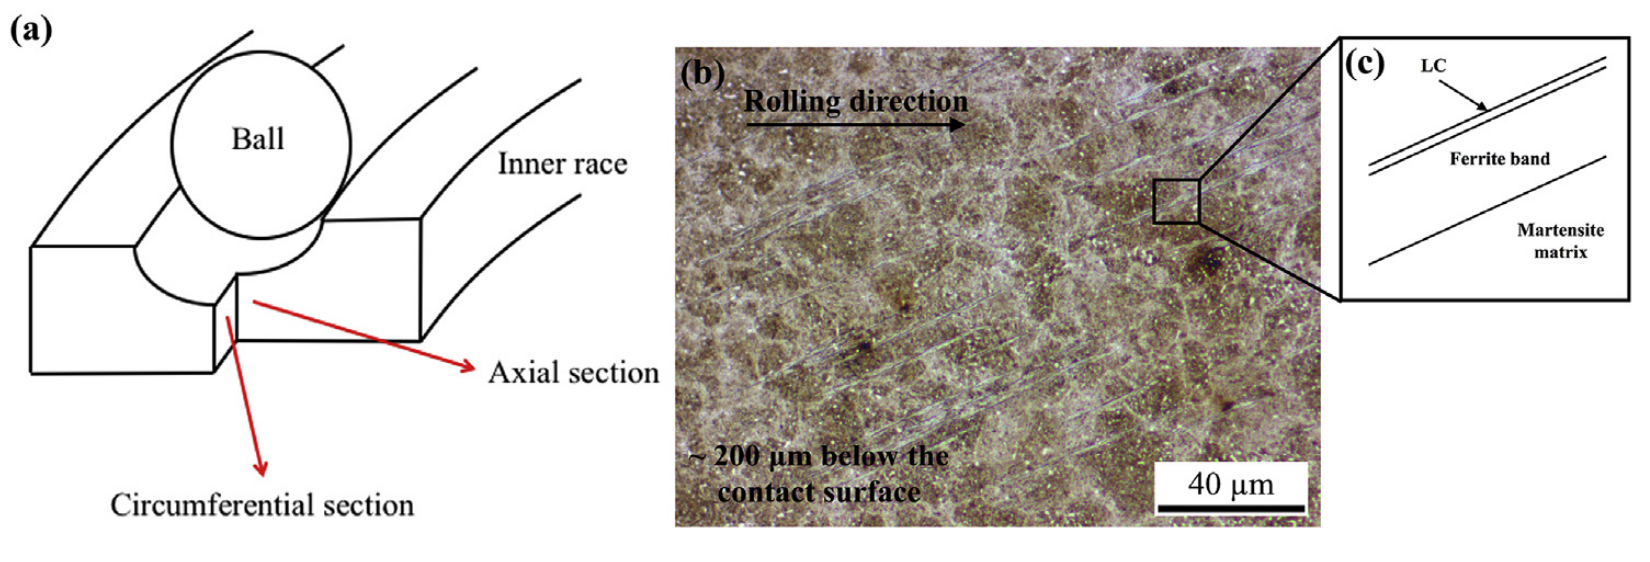
\includegraphics[width=.9\linewidth]{/home/tigany/Documents/docs/Management/Images/der_picture_fu.png}
\caption{Diagram of DER location within a bearing and its characteristics, taken from \cite{Fu2017}. (a) Axial and circumferential sections of a bearing inner ring. (b) Circumferential section of a bearing inner ring under optical microscope, where ferrite bands (white etching bands) are formed in the subsurface. (c) Diagram showing the structure of a WEB consisting of a ferrite band and a LC adjacent to it. One can see the DER region is composed of regions of ferrite interspersed in the parent martensite with lenticular carbides bordering the ferrite bands. \label{fuderpicture}}
\end{figure}


Decay of the martensitic microstructure is complex, with observation of many different
phenomena. Martensite transforms to ferrite microbands as a result of strain localization
\cite{Fu2017,il_micros_alter_rollin_contac_fatig,jonesil_metal_obser_ball_bearin_fatig_phenom,70_micros_microh_resid_stres_chang,Swahn1976,Voskamp1997,voskamp97_state_resid_stres_induc_by,polonsky95_white_etchin_band_format_rollin_bearin,vsmelova17_elect_micros_inves_micros_alter}. Residual
carbides, untouched at the start of DER formation, gradually dissolve within ferrite and
martensite \cite{70_micros_microh_resid_stres_chang,Swahn1976,Osterlund_1980}. Further RCF
progression leads to the formation of low and high angle ferrite features, White Etching Bands
(WEBs), composed of nanocrystalline \cite{Voskamp1997,Osterlund_1980,Mitamura_2007} and elongated
ferrite \cite{vsmelova17_elect_micros_inves_micros_alter}. Lenticular carbides precipitate at the
boundaries of these ferrite bands \cite{Swahn1976,Osterlund_1980}. Thickening of these carbides
occurs during DER development and is correlated with WEB growth
\cite{Fu2017,fu17_strain_induc_marten_decay_bearin,Warhadpande1_2013,Warhadpande2013}. Reductions in
dislocation density in nanocrystalline (heavily deformed) ferrite have been observed in the later
stages of DER formation \cite{skf2019,voskamp80_gradual_chang_resid_stres_micros}.



Carbon migration is thought to be the mechanism by which this degradation occurs, but it is not
definitively known how or where carbon migrates with the onset of DER formation. The key questions
are: where does excess carbon from the martensitic matrix find itself when the structure decays to
low solubility (0.02 wt\%) ferrite? and how is the carbon transported, given its low diffusivity in
martensite/DER phases
\cite{hashemi11_stren_hardn_statis_correl_api_x65_steel}? 


Fu \emph{et al.} propose that carbon atoms inside the martensite would segregate to
pre-existing/residual carbides, increasing their size
\cite{fu17_strain_induc_marten_decay_bearin}. This theory was successfully applied to the
growth of lenticular carbides \cite{Fu2017}, however, problems arise with the application to
temper carbide growth: if carbides were to form in martensite, they should follow the
Bagaryatskii/Isaichev orientation relationship, but observations suggest a lack of any orientation
relationship \cite{Bhadeshia2018}. Temper carbides residing within DERs have irregular
shapes/diffuse boundaries, which are seemingly due to the incomplete \emph{dissolution} of \emph{temper}
carbides, which is at odds with the theory of Fu \emph{et al.}.

A plausible mechanism for carbon migration is that it is driven by dislocation glide, which is as
follows
\cite{Fu2017,Swahn1976,voskamp97_state_resid_stres_induc_by,fu17_strain_induc_marten_decay_bearin,Warhadpande1_2013,Warhadpande2013}. Due
to the high dislocation density exhibited in martensite, carbon segregates to dislocations in
Cottrell atmospheres, causing pinning. Strain generated by cyclic stresses allow dislocations to
escape their carbon rich environment. The free dislocations re-attract carbon, allowing the
Cottrell atmospheres to reform, subsequently re-pinning the dislocations, creating a net carbon
flux.  This mechanism allows for the movement of carbon during the martensite-ferrite transition,
while also explaining how excess carbon can move from the ferrite phases to lenticular carbides at
the boundaries, describing the process behind both WEB growth and carbide thickening. Moreover, it
explains the dissolution of residual carbides, both in ferrite WEBs and martensite, due to
dislocation rearrangement and pile ups at the carbide interface drawing carbon atoms out, due to a
more favourable binding to dislocations. However, as to how this process occurs on the atomistic
scale, or if it is indeed feasible, is unknown.



Experimentally probing dislocation-assisted carbon migration has proven difficult and inconclusive. Work needs to be done
to understand dislocation-carbon interactions; more specifically: how dislocations move carbon
within the temperature and stress regimes experienced during operation; where carbon is
transported to and what the resultant dislocation networks are. 


To shed light on this mechanism, a multi-scale modelling approach can be
used. Atomistics can provide information of the 2d Peierls energy landscape which dislocations are
subject to in iron; and how this landscape is modified by the binding of carbon to
dislocations. This data can be used in a line tension model of a dislocation to determine the
kink-pair formation energies of dislocations as a function of carbon content and stress. Finally,
one can use a kinetic Monte Carlo (kMC) model of dislocation glide by thermally activated
kink-pair nucleation, in an environment of carbon. From this last stage of coarse-graining, one
can determine in which regimes of temperature, stress and carbon concentration,
dislocation-assisted carbon migration becomes a feasible mechanism behind DER formation, with
predictions of dislocation velocity, dislocation configurations and where carbon moves with
dislocation glide. 

In this report, we will focus on the atomistic portion of this project,
directed at understanding dislocation-carbon interactions at the atomistic scale in ferrite (bcc
iron).
With further knowledge of the fundamental mechanism behind DER formation, we can hope to suppress
dislocation motion in the martensitic matrix, mitigating failure by RCF.



\section{Computational Method}
\label{sec:orge279d73}


We use the tight-binding model of Paxton and Elsässer \cite{Paxton2013}, which has been shown to
describe the binding energies of carbon complexes in bcc iron, in good agreement with DFT
calculations. This model reproduces the two screw dislocation core structures---the easy and hard
\(1/2\langle 111 \rangle\) cores---exhibited in bcc iron. Study of both is crucial to understanding
solute-dislocation interactions. The easy core is the ground state in pure iron, but solutes, such
as hydrogen and carbon, have been shown to reconstruct this core into the hard core
configuration \cite{Ventelon2015,itakura13_effec_hydrog_atoms_screw_disloc}. Computationally cheaper
models, which do not incorporate quantum mechanics, such as the EAM, cannot reproduce these
behaviours.


\subsection{Peierls Potential}
\label{sec:org60394bf}

To determine the Peierls potential of the \(1/2\langle 111 \rangle\) screw dislocation, we followed the
procedure detailed in Itakura \cite{Itakura2012}. Quadrupolar arrays of dislocations were
constructed by placing dislocations of antiparallel \(1/2\langle 111\rangle\) Burgers vectors in an "S"
arrangement \cite{Clouet2012}, with initial displacements determined by anisotropic elasticity
solutions. See figure \ref{fig:dislocationschematics}, left. A quadrupolar arrangement minimises
the stress each dislocation experiences in the simulation. These displacements were modified to
be periodic, thereby removing artificial stacking faults which would appear between periodic
images after introduction of the dislocation dipole. This was achieved by the subtraction of a
linear error term from the superposition of displacement fields arising from the dislocations in
the simulation cell and its periodic images \cite{vasilybulatov2006}. To accommodate for the
internal stress upon introduction of a dislocation dipole into the simulation cell, an elastic
strain was applied to the cell, resulting in an additional tilt component to cell vectors
\cite{Clouet2012,vasilybulatov2006}. Simulation cells were constructed with different initial core
positions, which were sampled from the triangular region "EHS" (easy, hard and split) core
positions, as detailed in figure \ref{sampledpositions}. To fix the dislocation positions during
relaxation, the three atoms surrounding the easy core, for each dislocation, were fixed in \(Z\)
coordinate during relaxation, where \(Z\) is a \(\langle 111 \rangle\) direction, along the dislocation line. The
k-point sampling mesh for each of these cells was 5x5x30.


        \begin{figure}
    \begin{tabular}{cc}
	     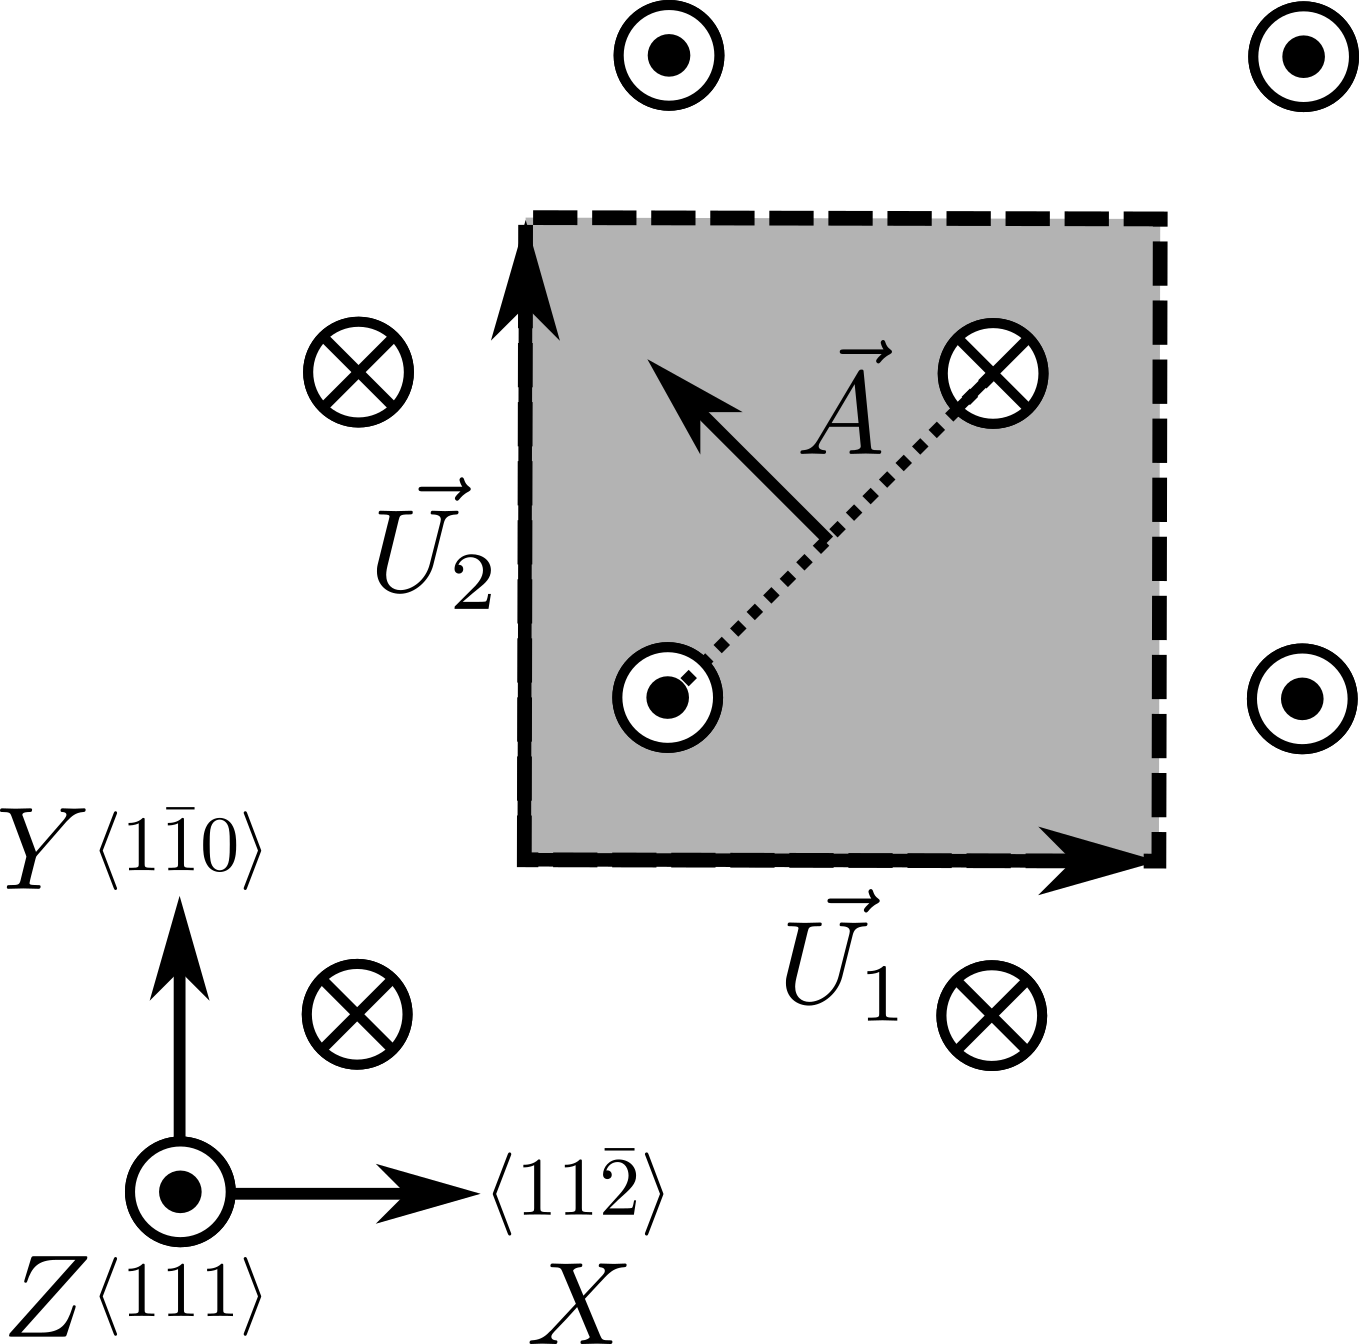
\includegraphics[width=0.5\textwidth]{Images/s_arrangement_quadrupole.png} &
             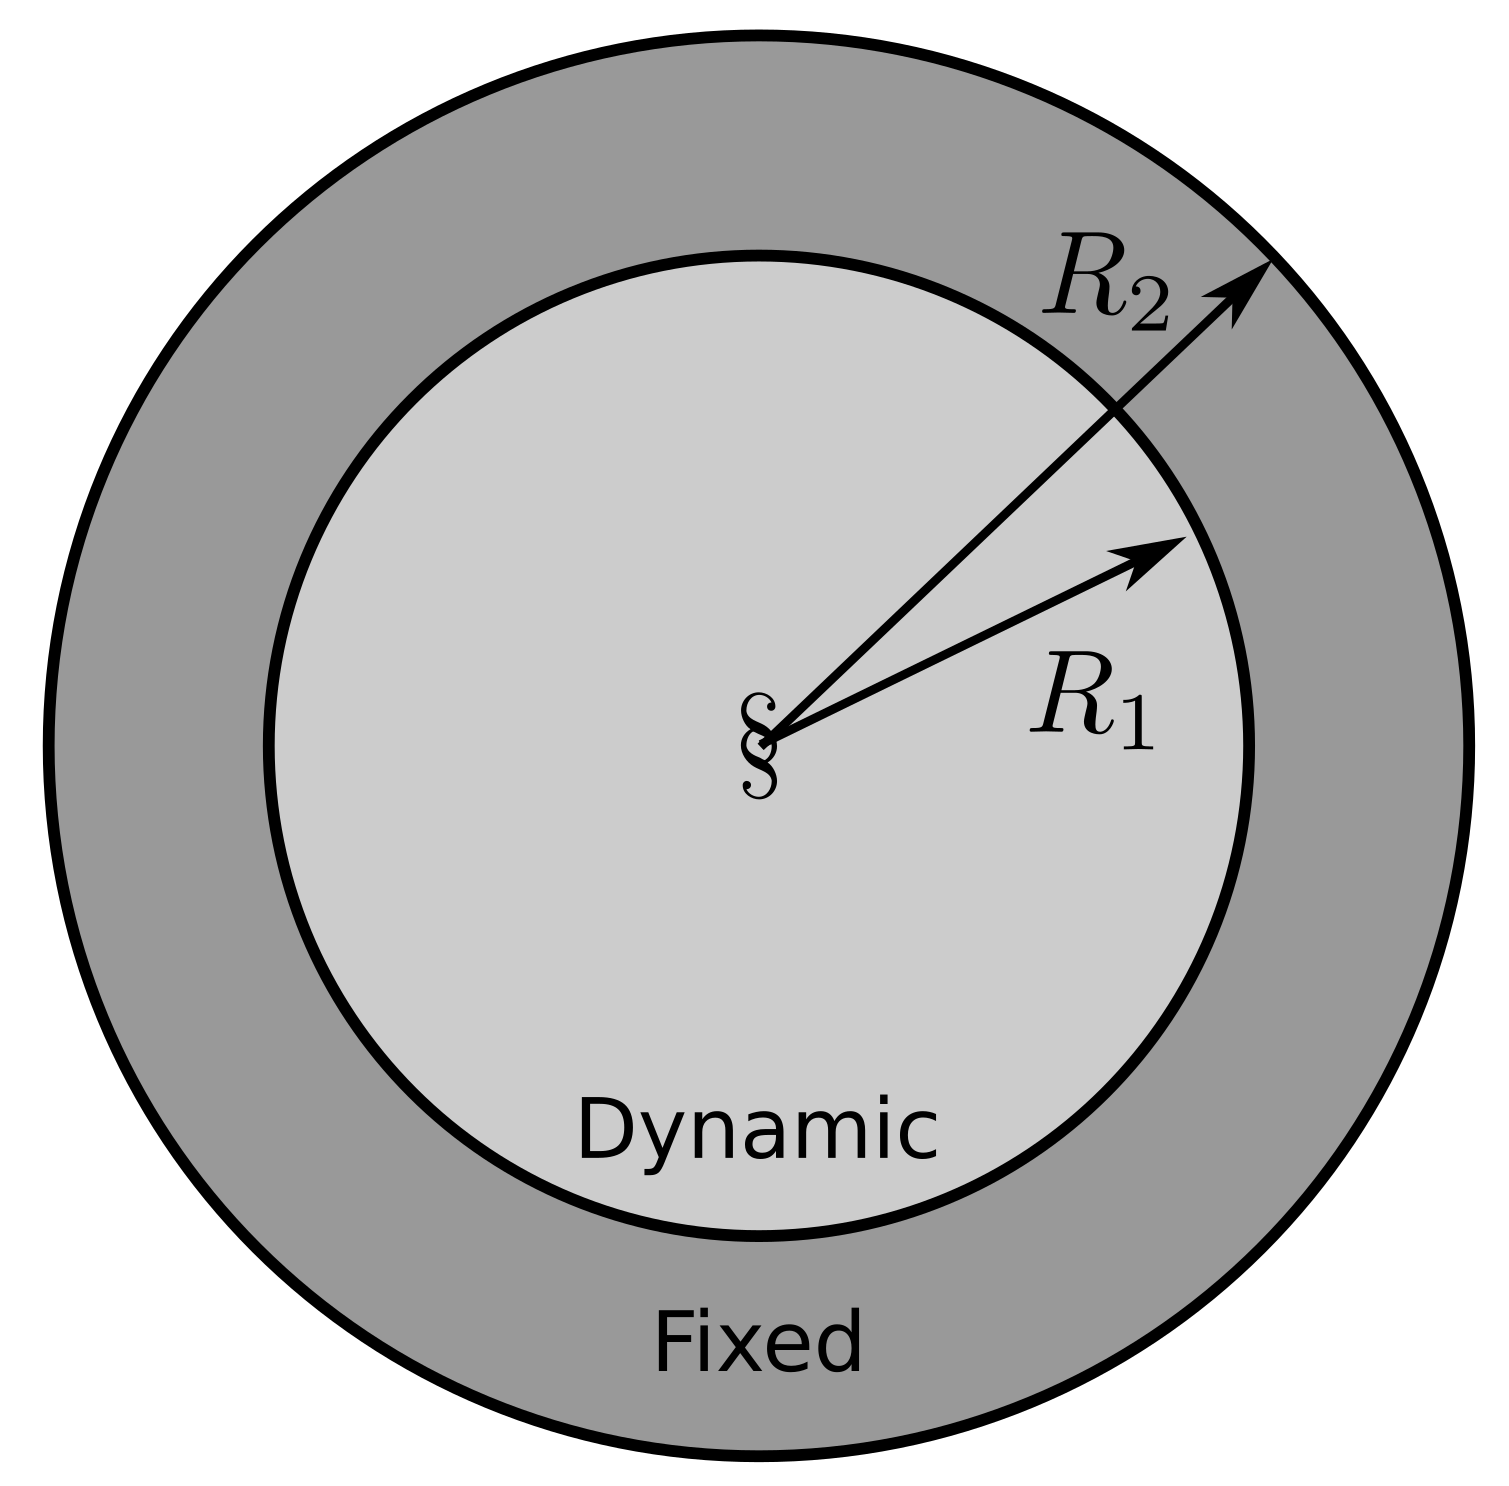
\includegraphics[width=0.45\textwidth]{Images/cluster_method_schematic.png}  \\
    \end{tabular}		
\caption{Schematics of dislocation simulation methods. Left: quadrupolar arrangement of dislocations in a simulation cell (grey square). This arrangement  minimises the stress experienced by each dislocation in a periodic simulation. Cell vectors $\vec{U}_1$ and $\vec{U}_2$ are shown; $\vec{A}$ defines the cut plane between the dipoles. The dislocation positions, and their corresponding burger's vector direction, are denoted by the symbols $\otimes$ and $\odot$, which are antiparallel to each other. Tilt components added to cell vectors to accomodate for the plastic strain are not shown. Right: cluster method, where atoms are displaced according the displacement field from the screw dislocation at the centre of the cluster, denoted by "\S". Atoms in the annulus $R_2 - R_1$ are fixed in position to the anisotropic elasticity solutions. Within $R_1$, all atoms can relax. Periodicity is only imposed in the $Z$ direction.}
	\label{fig:dislocationschematics}
    \end{figure}



        \begin{figure}
    \begin{tabular}{cc}
	     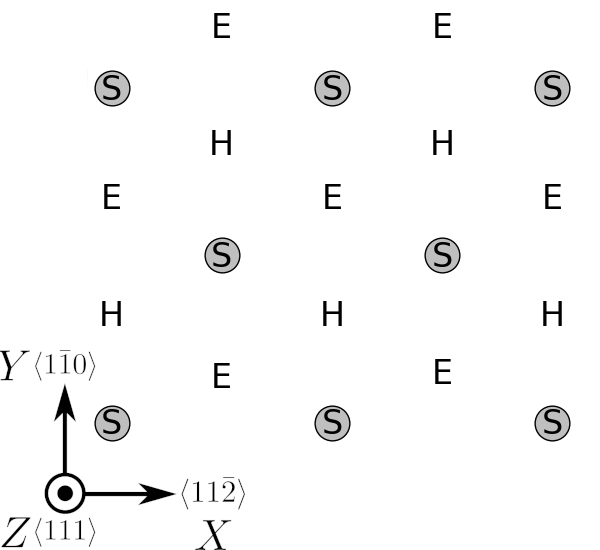
\includegraphics[width=0.5\textwidth]{Images/hardeasycoreatomdiagram_coordnew.png} &
             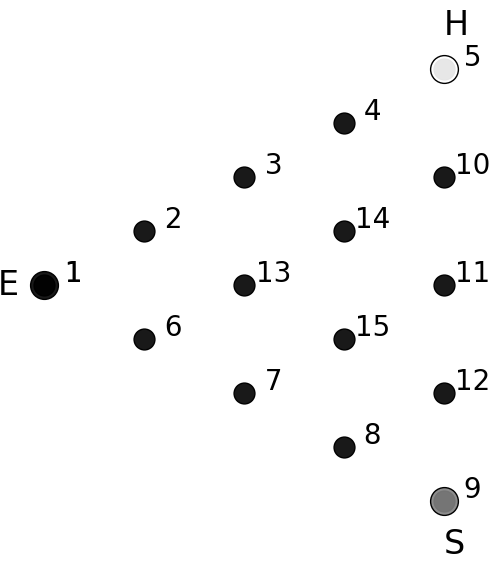
\includegraphics[width=0.45\textwidth]{Images/peierls_potential_positions_tbe.png}  \\
    \end{tabular}		
\caption{Diagrams of dislocation core positions. "E", "H" and "S" correspond to the easy, hard and split core positions respectively. Left: core positions as seen along the $Z=\langle 111 \rangle$ direction, along the dislocation line. Atomic positions are shown as grey circles. Right: positions sampled within the triangle EHS used to determine the Peierls potential.  \label{sampledpositions}}
	\label{fig:peierlspot}
    \end{figure}


The interaction energy between the dislocation dipole and periodic images was defined differently
to Itakura \cite{Itakura2012}. We followed the prescription of Bulatov and Cai \cite{vasilybulatov2006} to
find a regularised interaction energy, which is independent of truncation limit, in contrast to
the formulas quoted in Itakura's papers. Details can be found in section \ref{sec:Ainteractionenergy}.




The Peierls potential \(\Delta E_{\text{P}}^i\), for an isolated dislocation at the \(i^{\text{th}}\) core
position, can be calculated from
\begin{equation}
 \Delta E_{\text{P}}^i = \Delta E_{\text{tbe}}^{i} - \Delta E_{\text{INT}}^{i} ,\label{eq:peierlspot} 
 \end{equation} 
where \(\Delta\) refers to quantities, per dislocation, relative to the relaxed easy core configuration
(labelled as E/1, as in figure \ref{sampledpositions}). \emph{e.g} \(\Delta E_{\text{tbe}}^{i} = \frac{1}{2} (
   E_{\text{tbe}}^{i} - E_{\text{tbe}}^{\text{E}} )\) is the difference in energy, per dislocation, between
a relaxed cell which has the two dislocation cores placed at position \(i\), \(E_{\text{tbe}}^{i}\), and a relaxed
cell which has the two cores placed in easy core positions \(E_{\text{tbe}}^{\text{E}}\), divided by the number of
dislocations in each of the simulation cells. Dislocation-dislocation interaction
energies are included in this term, due to dislocations in the simulation cell---and
periodic images---interacting with each other, as can be readily seen in figure
\ref{fig:dislocationschematics}. To model the energy landscape of an isolated dislocation, these
interaction energies must be subracted, which is achieved by the correction term \(\Delta E_{\text{INT}}^{i}
   = \frac{1}{2} ( E_{\text{INT}}^{i} - E_{\text{INT}}^{\text{E}} )\).

\subsection{Preliminary calculations}
\label{sec:orga74954c}
To determine the binding energy of carbon to dislocations, we used the cluster method, as shown
in figure \ref{fig:dislocationschematics}, right. Simulation
cells consisted of a cylindrical cluster of atoms, with a single dislocation introduced into the
centre using displacements from anisotropic elasticity solutions. Each of the clusters were
centred on the easy or hard core positions. The cluster of atoms was split into two regions: a
central region of dynamic atoms with radius \(R_1\), and an annulus of atoms, between \(R_1\) and \(R_2\),
which were fixed in position to the displacements from anisotropic elasticity.


To confirm the anisotropic elasticity solutions were correct, we compared the
displacements against the analytic solutions to the straight screw dislocation, as given in Hirth
and Lothe \cite{anderson2017theory}. Furthermore, energy scaling relations were verified. We
inserted dislocations into cells of varying radii: \(R_1 = x\sqrt{2}a_{\text{bcc}}\), and \(R_2 =
   (x+1)\sqrt{2}a_{\text{bcc}}\), where \(x \in \{2\dots5\}\). The excess energy
was defined as the energy difference of a cell with a dislocation inserted, \(E_{\text{d}}\), with
respect to a perfect cell reference energy of the same geometry,

\begin{equation}
 E_{\text{excess}} =   E_{\text{core}} + E_{\text{elastic}} = E_{\text{d}} - E_{\text{perfect}}   ,\label{eq:excessenergy}
 \end{equation} 
where
\(E_{\text{elastic}} = ( \mu b^2 / 4\pi )\text{ln}(R/ r_c)\), with \(R = R_2\) and \(r_c = b\).

Initially, large cells of \(R_1 = 6\sqrt{2}a_{\text{bcc}}\), and \(R_2 =
   7\sqrt{2}a_{\text{bcc}}\) with depth of single burger's vector, were relaxed
for both the easy and hard cores, which consisted of 522 and 540 atoms
respectively. The three atoms surrounding the core were constrained to only
relax in \(X-Y\) plane, to fix the dislocation upon relaxation. 
The k-point sampling mesh for each of these cells was 1x1x24.

From the relaxed cells, a smaller region of 174 atoms, with \(R_1 = 3\sqrt{2}a_{\text{bcc}}\), and \(R_2
   = 4\sqrt{2}a_{\text{bcc}}\), was cut from the dynamic regions. This smaller cell was extended to a
thickness of 3\(b\) in the \(Z\) direction. Carbon interstitials were inserted into octahedral sites
near the dislocation core, in the middle layer. Exploiting reflection and rotational symmetry,
only 10 interstitial sites needed to be used to obtain the binding energies of carbon \(\sim2\) b from
the core, denoted by iH\(j\) and iE\(j\), where \(j \in \{1\dots10\}\). The final binding sites are denoted
by H\(k\) and E\(j\), where \(k \in \{1\dots7\}\). The three atoms surrounding the core in the first and
third layers were again constrained to relax only in the \(X\) and \(Y\) directions. No such
constraints were imposed on the middle layer.


\subsection{Fe-C binding energies}
\label{sec:orgd5b4a47}
We calculated the carbon-dislocation binding energies as in Itakura
 \cite{itakura13_effec_hydrog_atoms_screw_disloc}.

The binding energy is given by 
\begin{equation}  
E_b = E_{\text{d+C}} + E_{\text{perfect}}- E_{\text{d}} - E_{\text{C ref.}},    
\end{equation}

where \(E_{\text{d+C}}\) is the total energy of a relaxed cluster with a
carbon interstitial and a dislocation, \(E_{\text{d}}\) is the total
energy of a relaxed cluster with a dislocation and \(E_{\text{C
    ref.}}\) is the total energy of a relaxed perfect cluster with a single carbon in
an octahedral site. A positive binding energy indicates favourable binding.

The zero-point energy (ZPE) is calculated as in Itakura. Details can be found in \ref{sec:zeropointenergy}. 
The ZPE corrected binding energy is given by 
\[ E^{\text{Z}}_{b} = E_b + \Delta E_z,  \]
where \(\Delta E_z = E_z - E_{z}^{\text{C ref.}}\) and \(E_{z}^{\text{C ref.}} = 202.5 \text{meV}\) is the zero-point energy of carbon
situated in an octahedral site in a perfect cluster of the same size. 

\subsection{Analysis of carbon concentration along dislocation}
\label{sec:org66b1035}

Using the Fe-C binding energies, one can predict the equilibrium carbon concentration of a carbon
binding site \(c_d\), under the assumption that carbon atoms around the core are sufficiently spaced such that intersite
interaction energies are negligible \cite{Ventelon2015}.

The concentration is given by 

\begin{equation}
\frac{ c_d^{i} }{1 -  c_d^{i} } = \frac{ c_{\text{bulk}}^{} }{1 - c_{\text{bulk}} } \text{exp} \Big( 
\frac{E_{\text{b}}^i}{k_{\text{B}}T}  \Big),    \label{eq:cd}
\end{equation}
where \(i\) denotes the \(i^{\text{th}}\) carbon binding site, with \(E_{\text{b}}^{i}\), being the
corresponding dislocation-solute binding energy (in the convention of attraction
denoting a positive binding energy). \(c_d^{i}\) is the average concentration of the \(i^{\text{th}}\) carbon
site bound to the dislocations. \(c_{\text{bulk}}^{}\) is the carbon concentration in the bulk, with
\(c_{\text{nom}}^{}\) the nominal carbon concentration per Fe atom.


In a given volume \(V\), the number of carbon sites along the dislocation cores is \(N_d = \rho V/b\),
with \(\rho\) the dislocation density, and the number of octahedral sites is \(N_{\text{oct}} =
    6V/a_{\text{bcc}}\). This imposes constraints on the carbon concentrations: \(N_{\text{oct}}
    c_{\text{bulk}}^{} + N_d c_d = N_{\text{oct}} c_{\text{nom}}/3\), where the factor of 3 is because there are
three octahedral sites per Fe atom in the bcc lattice. Using this relation, equation \ref{eq:cd}
can be solved self-consistently to give the carbon concentration around the core, as a function
of nominal carbon concentration and temperature. The nominal carbon concentration was taken to
be the maximum solubility of ferrite in the DER region, 0.02 wt\% \(\approx 433\) appm
\cite{hashemi11_stren_hardn_statis_correl_api_x65_steel}. Calculations of 10 and 1000 appm were
also performed. The dislocation density was varied between \(1\times10^{12}\), \(1\times10^{14}\) and \(5\times10^{15}\), to
see the effects of low densities up to the upper bound of dislocation densities \(\sim5\times10^{15}\)
found in Fe-0.61wt\%C martensite \cite{morito03_disloc_densit_within_lath_marten}.


\subsection{Progression to Line Tension Model}
\label{sec:org918ea48}

From the atomistic calculations of the Peierls potential and carbon-dislocation binding energies, one can make a
line tension model of a dislocation from which we can obtain the kink-pair formation energies as
a function of stress and carbon content.  This model views the dislocation as an elastic string
which moves on the Peierls potential \(\Delta E_{\text{P}}\).

The dislocation is modelled as a discretised line, with layer labels \(j\). The energy of the
dislocation line is given by:

\[ E_{\text{LT}} = \frac{K}{2} \sum_j (\vec{P}_j - \vec{P}_{j+1} )^2  + \sum_j \Delta E_{\text{P}}  (\vec{P}_j) +
   (\sigma \cdot \vec{b}) \times \vec{l} \cdot \vec{P}_j  - \sum_{j,k} E_{\text{C}} (|\vec{P}_j-\vec{P}_k^{}^{\text{C}}|), \]

where \(K\) is a constant calculated from the model, \(\Delta E_{\text{P}}\) is the Peierls potential, \(\sigma\) is
the stress applied and \(\vec{b}\) is the burger's vector, with the dislocation line sense given by
\(\vec{l}\). \(\vec{P_{j}}\) corresponds to the dislocation core position in a given
layer. \(E_{\text{C}} (|\vec{P}_j-\vec{P}_k^{}^{\text{C}}|)\) is the binding energy of a particular carbon
\(k\), at position \(\vec{P}_k^{\text{C}}\), to a dislocation core positioned at \(\vec{P}_j\). The kink-pair
formation enthalpies can then be found using the NEB/String method, to find the height of the transition-state
barrier. 

\section{Results}
\label{sec:org39312e5}

\subsection{Peierls Potential}
\label{sec:orgf7e4f73}

        \begin{figure}
    \begin{tabular}{c}
	     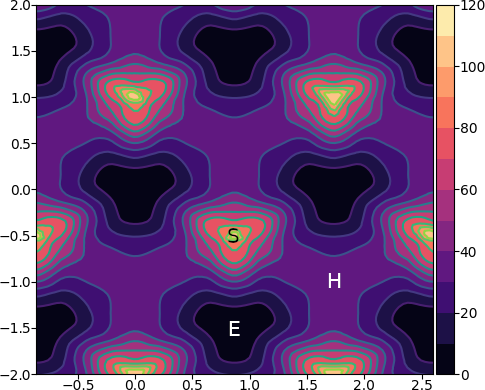
\includegraphics[width=0.8\textwidth]{Images/itakura_dislocation_energy_landscape_2_labelled.png} \\
             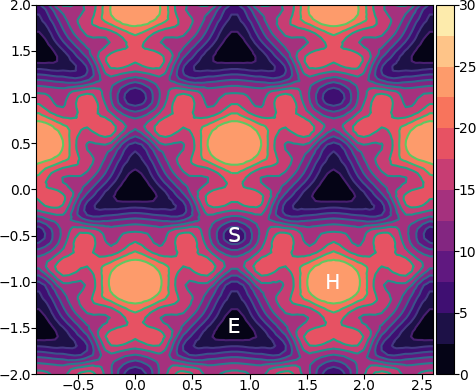
\includegraphics[width=0.8\textwidth]{Images/tbe_dislocation_energy_landscape_pure_labelled.png}  \\
    \end{tabular}		
\caption{Comparison of 2d Peierls potentials of the $1/2\langle 111\rangle$ screw dislocation between DFT \cite{Itakura2012} (top) and tight-binding (bottom). Energy scale is in meV. "E", "H" and "S" correspond to easy, hard and split core positions respectively, with the latter also corresponding to atomic positions. The relative energies between the different core positions is smaller in tight-binding compared to DFT. The split core as seen in tight-binding is reminiscent of EAM potentials, where the split core energy is lower than that of the hard core. The discrepancy is probably due to an insufficient repulsion at close range within the tight-binding model.}
	\label{fig:peierlspot}
    \end{figure}



Comparison of 2d Peierls potentials of the \(1/2\langle 111 \rangle\) screw dislocation
between DFT and tight-binding can be found in figure \ref{fig:peierlspot}, with data found in
table \ref{tab:peierlspot}. The sampled energies were interpolated using 2d cubic splines. The
relative energies between the different core positions was found to be smaller in
tight-binding compared to DFT. This is an artifact of the model, which has been reproduced
in NEB calculations of the \(1/2\langle 111\rangle\) screw dislocation Peierls barrier: the
tight-binding Peierls barrier is approximately half that of DFT \cite{Simpson2019}. The split
core energy is lower than that of the hard core, which is reminiscent of EAM potentials
\cite{Itakura2012}. Some of this discrepancy can be attributed to the to erroneous interaction
term included by Itakura, as detailed above---interaction energies can become arbitrarily
high, if not made independent of truncation limit---but likely there are effects in DFT
which are not encapsulated fully within the tight-binding description, such as a lack of
core electron repulsion upon deformation of the lattice, which would increase the relative
energy difference. Consequences of this discrepancy on future kMC simulations are discussed
in section \ref{sec:discussion}.


\begin{table}[htbp]
\caption{Table of energies used to calculate the Peierls potential. All values in meV. \(\Delta E_{\text{P}}^{\text{DFT}}\) values taken from \cite{Itakura2012}. \label{tab:peierlspot}}
\centering
\begin{tabular}{rrrrr}
Pos & \(\Delta E_{\text{INT}}\) & \(\Delta E_{\text{tbe}}\) & \(\Delta E_{\text{P}}\) & \(\Delta E_{\text{P}}^{\text{DFT}}\)\\
\hline
1 & 0 & 0 & 0 & 0\\
2 & -0.7 & 7.3 & 7.9 & 3.2\\
3 & -1.4 & 16.0 & 17.4 & 19.2\\
4 & -2.0 & 22.2 & 24.2 & 31.1\\
5 & -2.5 & 24.8 & 27.4 & 39.3\\
6 & -3.3 & 3.0 & 6.3 & 11.5\\
7 & -6.5 & 7.1 & 13.6 & 39.9\\
8 & -9.6 & 13.0 & 22.6 & 75.2\\
9 & -12.5 & 5.4 & 17.9 & 108.9\\
10 & -4.8 & 22.1 & 26.9 & 34.8\\
11 & -7.2 & 18.2 & 25.4 & 37.9\\
12 & -9.8 & 14.0 & 23.8 & 60.7\\
13 & -3.8 & 11.5 & 15.3 & 17.6\\
14 & -6.9 & 15.1 & 22.0 & 29.9\\
15 & -4.3 & 18.6 & 22.9 & 39.7\\
\end{tabular}
\end{table}


\begin{figure}[htbp]

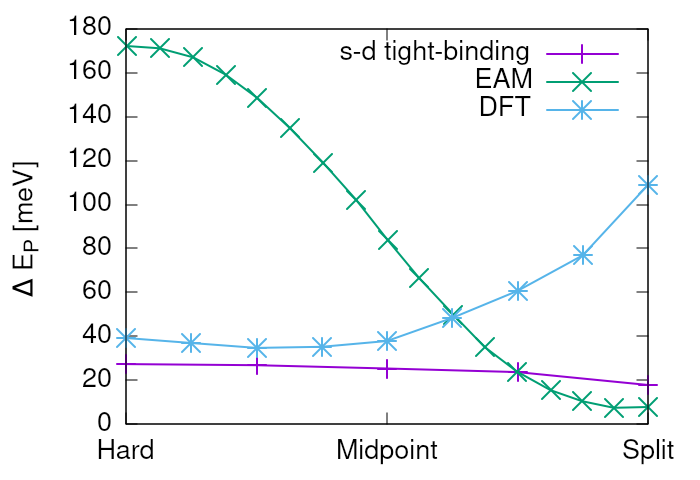
\includegraphics[width=0.8\textwidth]{Images/hard-split_transition.png}
\caption{Peierls potential along the hard-split line. One can see in \(s\text{-}d\) tight-binding model is similar to the EAM potential of Mendelev \cite{Mendelev2003}: it decreases constantly from the hard core to the split core, which will result in a kink shape which goes through the split core position. In DFT one finds a saddle point between the hard core and the midpoint, in which a kink in the transitional state will go through. \label{hardsplittransition}}
\end{figure}



The expected transitional kink shape from this Peierls potential may differ compared to DFT, with
dislocation core positions possibly being situated closer to/at the split core position, similar
to EAM potentials \cite{Itakura2012}. Following the Peierls potential along the H-S direction,
figure \ref{hardsplittransition}, we see that the Itakura potential has a saddle point, whereas in
\(s\text{-}d\) tight-binding there is not: the Peierls potential decreases monotonically
from the hard core to the split core position. However, calculation of the Peierls barrier between
two easy core positions in the canonical \(d\text{-band}\) version of this tight-binding model
(where \(s\text{-}d\) hybridisation and non-orthogonality are simply turned off) found core
positions of the transitional kink state to go through the metastable point, similar to DFT
\cite{Simpson2019}. Furthermore, the canonical \(d\text{-band}\) model produces structural energy
differences and elastic constants which are closer to values in literature than the \(s\text{-}d\) model
\cite{Paxton2010}; as such, it could provide a better description of Fe-Fe interactions, and the
Peierls potential, by extension. To verify this, recalculation of the Peierls potential using the
canonical model will need to be undertaken.

\subsection{Preliminary calculations}
\label{sec:org5bbdf2b}


To validate the cluster simulation method, the excess energy, defined as the difference in energy
between a cell with a dislocation, and a perfect reference cell, was plotted as as function of
\(\text{ln}(R/r_c)\), where \(R = R_2\) of the cluster and \(r_c = b\), as seen in
figure \ref{lnrdep}. In isotropic elasticity theory, this should give a linear dependence where the gradient
corresponds to \(\mu b^2 / 4\pi\), with the \(y\) intercept corresponding to the
core energy \(E_{\text{core}}\). This is well reproduced by our model, except at low \(\text{ln}(R/r_c)\)
as expected, where the cell size is not large enough to accommodate for sufficient relaxation of
the dislocation core, increasing the core energy, which is not accounted for in elasticity theory.


\begin{figure}[htbp]
\centering
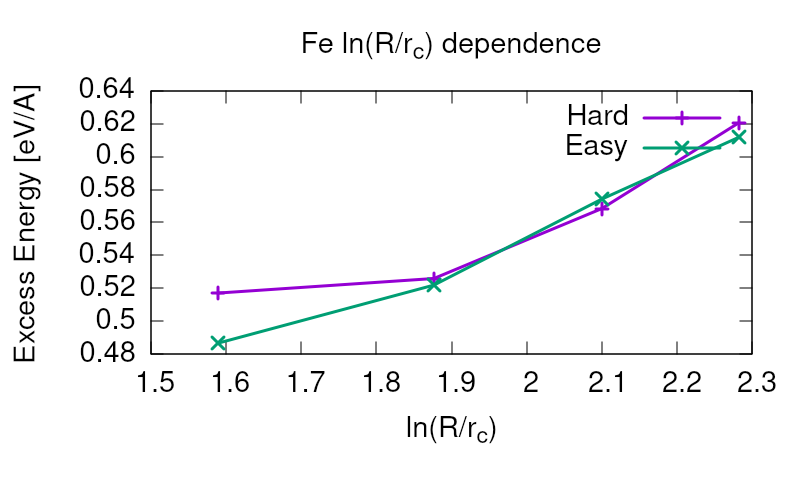
\includegraphics[width=.9\linewidth]{/home/tigany/Documents/docs/Management/Images/img_fe_size_dependence_on_log_of_core_radius.png}
\caption{Excess energy of dislocation clusters with differing radii for both the easy and hard core configurations. The prediction from elasticity theory is given by the black, dashed line. Deviation of both cores occur when cell size is small, creating an increase in the core energy, which elasticity theory cannot account for. \label{lnrdep}}
\end{figure}




The energy cost to transform from the easy to the hard core can be estimated by
the difference in excess energies between the cores in the limit of
\(\text{ln}(\frac{R}{R_0}) \rightarrow 0\). At the smallest measured value, one finds that the core energy
difference \(\Delta E_{\text{core}}^{\text{Easy-Hard}} = 76\) meV/b, which is in good agreement with the DFT
value of 82 meV/b \cite{Itakura2012}.



\subsection{Fe-C binding energies}
\label{sec:org14782f5}



As found in DFT simulations by Ventelon \cite{Ventelon2015}, when a carbon was placed in the
vicinity of a relaxed easy dislocation core---in either of the two nearest, distinguishable,
octahedral sites---a spontaneous reconstruction of the dislocation core occurred: from easy to
hard. Upon reconstruction, the dislocation core moved to a neighbouring triangle, when looking
along the \(\langle 111\rangle\) direction, where the carbon found itself situated in the centre. This will be
called a prismatic site, as in Ventelon's paper. This confirms that both hard and easy
dislocation cores must be studied to fully understand screw dislocation behaviour in bcc iron.


The binding energies of carbon to both the hard and easy cores can be seen in table
\ref{tab:bindingenergies}, with the resulting distribution of carbon in figures
\ref{easybindingenergydist} and \ref{hardbindingenergydist}. The distribution of carbon strongly
depends on the type of core it finds itself situated near. The easy core only significantly
modifies the position of the iE1 site, to the E1 site, situated in the centre of an adjacent
triangle. All other sites are unaffected, so there is a one-to-one correspondence between all
\(\text{iE}j\) and \(\text{E}j\) sites, where \(j \in \{2\dots10\}\). There are carbon basins available close
to the triangular region containing the core, but not inside.

Carbon favours a prismatic site within the hard core (H1), which has the highest
binding energy, 1.29 eV, of all sites considered. There are no binding sites apparent in a triangular
annulus (of width \(a_{\text{bcc}}\sqrt{2}/2\)) surrounding the hard core triangle due to the
destruction/volume reduction of octahedral sites near the hard core. The initial octahedral
sites, iH1 and iH2 decay to the H1 site. Similarly, iH3 and iH4 decay to the H2 site, with iH9
and iH10 decaying to a H7 site. Relations between each of the sites is given in table
\ref{decayrelations}.


\begin{table}[htbp]
\caption{Decay relations between the initial and final sites upon relaxation of carbon intersitials around the hard core. \label{decayrelations}}
\centering
\begin{tabular}{ll}
Initial & Final\\
\hline
iH1, iH2 & H1\\
iH3, iH4 & H2\\
iH5 & H3\\
iH6 & H4\\
iH7 & H5\\
iH8 & H6\\
iH9, iH10 & H7\\
\end{tabular}
\end{table}


Note that interactions between carbon atoms around the core are not taken into account here:
figures \ref{easybindingenergydist} and \ref{hardbindingenergydist} are purely diagrammatic and not
what one expects the true distribution of carbon around a screw dislocation would be. Carbon is strongly
repulsive at first nearest-neighbour distances, which would modify each of these
distributions. 


\begin{figure}	
    \begin{tabular}{l}
 	          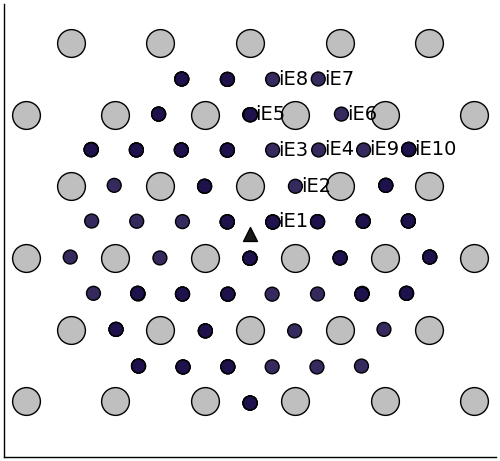
\includegraphics[width=0.7\textwidth]{Images/easy_core_fe_C_initial_positioning.png}  \\
 	          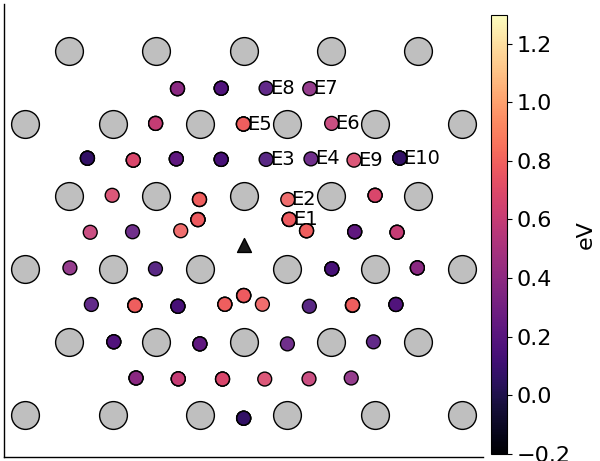
\includegraphics[width=0.85\textwidth]{Images/easy_core_fe_C_positioning_energies_e10_label.png}  \\

     	     \end{tabular}		
\caption{ Initial (top) and final (bottom) positions and binding energies (eV) of carbon around the easy core. Binding energies are not shown for the initial positions. Top: initial positions before relaxation. Bottom: final positions and binding energies after relaxation. The core was constrained by fixing the top and bottom three atoms surrounding each of the cores. As shown by Ventelon \cite{Ventelon2015}, the first and second closest octahedral sites to the hard core decay to a prismatic position inside the hard core. }
\label{easybindingenergydist}
   \end{figure}


\begin{figure}	
    \begin{tabular}{l}
 	          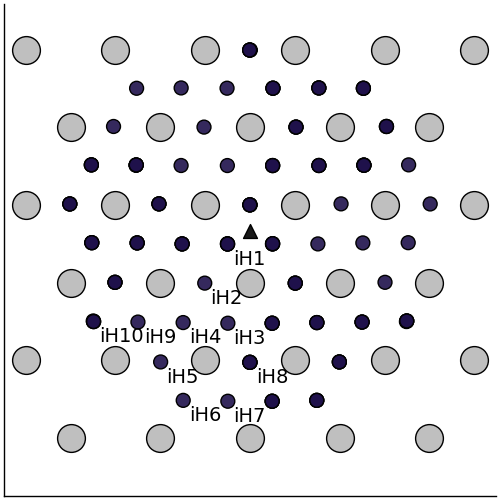
\includegraphics[width=0.7\textwidth]{Images/hard_core_fe_C_initial_positioning.png}  \\
 	          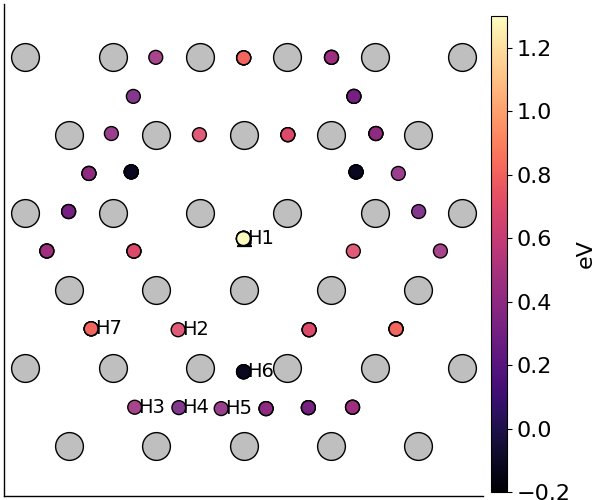
\includegraphics[width=0.85\textwidth]{Images/hard_core_fe_C_positioning_energies_h7_label.png}  \\

     	     \end{tabular}		
\caption{ Initial (top) and final (bottom) positions and binding energies (eV) of carbon around the hard core. The core was constrained by fixing the three atoms surrounding each of the cores in the top and bottom layers. As shown by Ventelon \cite{Ventelon2015}, the first and second closest octahedral sites to the hard core decay to a prismatic position inside the hard core. }
\label{hardbindingenergydist}
   \end{figure}




\begin{table*}
    \begin{tabular}{cccccc}
    \hline
Site Type & distance from core [b] & $E^{z}$ [eV] & $\Delta E^{z}$ [eV] & $E_b$ [eV] & $E_b^{z}$ [eV]  \\ 
     \hline
% 00        &                    --  &   0.203      &               0.000 &             &         --     \\
%           &                        &              &                     &             &                \\\hline
E1        &                   0.57 &   0.185      & 	     -0.018 &       0.793 &          0.775 \\
E2        &                   0.70 &   0.202      & 	     -0.001 &       0.793 &          0.793 \\
E3        &                   0.99 &   0.205      & 	      0.002 &       0.137 &          0.139 \\
E4        &                   1.21 &   0.208      & 	      0.005 &       0.229 &          0.234 \\
E5        &                   1.36 &   0.210      & 	      0.008 &       0.784 &          0.791 \\
E6        &                   1.66 &   0.209      & 	      0.007 &       0.597 &          0.603 \\
E7        &                   1.89 &   0.206      & 	      0.003 &       0.385 &          0.388 \\
E8        &                   1.77 &   0.203      & 	      0.000 &       0.177 &          0.178 \\
E9        &                   1.52 &   0.201      & 	      0.000 &       0.683 &          0.683 \\
E10       &                   1.95 &   0.202      & 	      0.000 &       0.067 &          0.067 \\ \hline
H1        &                   0.00 &   0.196      & 	     -0.006 &       1.298 &          1.291 \\
H2        &                   1.19 &   0.210      & 	      0.007 &       0.691 &          0.698 \\
H3        &                   2.12 &   0.209      & 	      0.007 &       0.461 &          0.467 \\
H4        &                   1.91 &   0.207      & 	      0.005 &       0.311 &          0.316 \\
H5        &                   1.80 &   0.208      & 	      0.006 &       0.403 &          0.409 \\
H6        &                   1.40 &   0.207      & 	      0.005 &      -0.119 &         -0.114 \\
H7        &                   1.35 &   0.206      & 	      0.006 &       0.825 &          0.819 \\

    \end{tabular}		
    \caption{Table of energies leading to the zero-point energy corrected binding energy using the cluster method for simulation of dislocation-carbon interactions. }
    \label{tab:bindingenergies}
\end{table*}

These binding energies agree well with experiment and atomistic/elastic calculations. EAM simulations
by Clouet \cite{Clouet2008,Becquart2007} found a maximum binding energy of 0.41 eV by calculating
the elastic dipole tensor within Eshelby theory. Hanlumyuang \emph{et al.} \cite{Hanlumyuang2010},
similarly conducted DFT and EAM calculations for the interaction energy 12\AA{} from the core, and
their calculations agreed with the continuum limit of Eshelby theory with a binding energy of
0.2 eV. In DFT calculations by Ventelon \cite{Ventelon2015}, the interaction energy of a carbon in a
hard core prism configuration was found to be 0.79 eV for a thickness in the \(Z\) direction of
3\(b\) (0.73eV for \(6b\))---in the convention that a positive binding energy indicates
attraction. This is significantly lower than the 1.29eV interaction energy of tight-binding.
This discrepancy can be partially explained by the fact that the cells have not been allowed to
relax with all degrees of freedom, as in the Ventelon results: the three atoms around the screw
core are fixed in \(Z\) to so the dislocation core position does not change upon relaxation. A
larger source of error is likely from the fitting of the tight-binding model itself. The
Peierls barrier of this \(s\text{-}d\) model of iron, necessary for Fe-C interactions, has been shown to be
half that found in DFT \cite{Simpson2019}, but the solution energies for
Fe-C defect complexes are well described. This implies there is insufficient repulsion between
Fe-Fe species upon deformation, leading to a larger resultant Fe-C binding energy from tight-binding.




\subsection{Analysis of carbon concentration along dislocation}
\label{sec:org2a5051a}

Variation of carbon concentration along the dislocation line for each of the binding sites can be
seen in figure \ref{cdhardeasy}. Due to the lower overall binding energies of carbon to the easy
core, the concentration of weakly bound sites occurred at a lower temperature. Dislocation
densities near the upper bound of what has been observed in martensite, \(\rho \approx10^{15}\), reduce
the temperature at which carbon concentration decreases around the dislocation core. Lower
nominal carbon concentrations cause carbon concentrations around the dislocation to decrease at a
lower temperature.

In the operating temperature range of \(40-90\deg\text{C} = 310-360\deg\text{K}\), we expect most hard
core sites are saturated. Given the high concentrations of the E1/E2 sites around the easy core
in this range, we expect all dislocations will be of the hard core type, due to reconstruction of
the easy core by the adjacent carbon.



\begin{landscape}
   \begin{figure}	
       \begin{tabular}{c}
      	        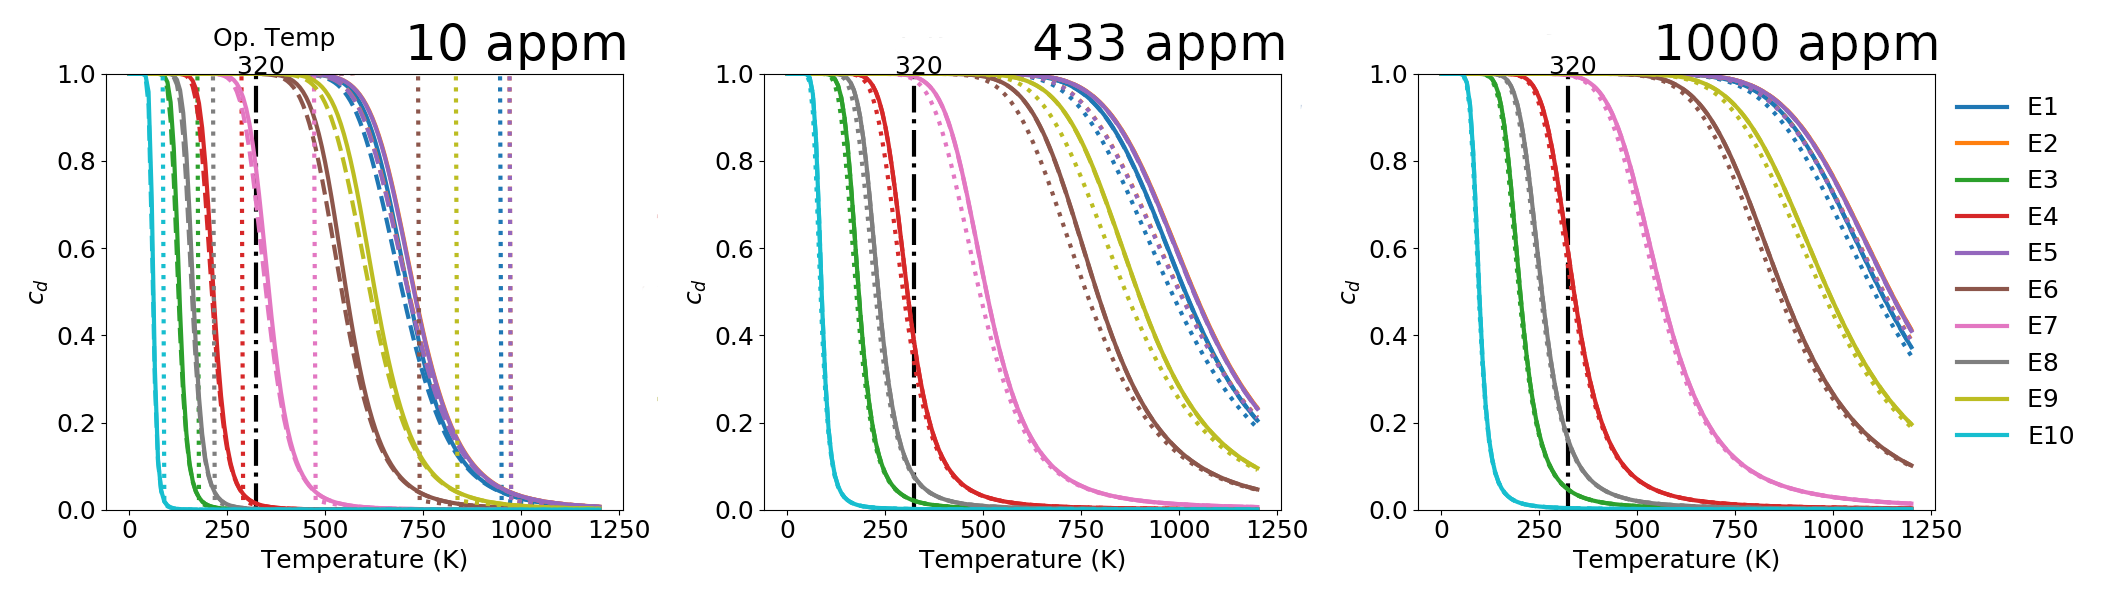
\includegraphics[width=1.65\textwidth]{Images/cd_easy_core_ferrite_sc_all_10_433_1000_appm.png}  \\
      	        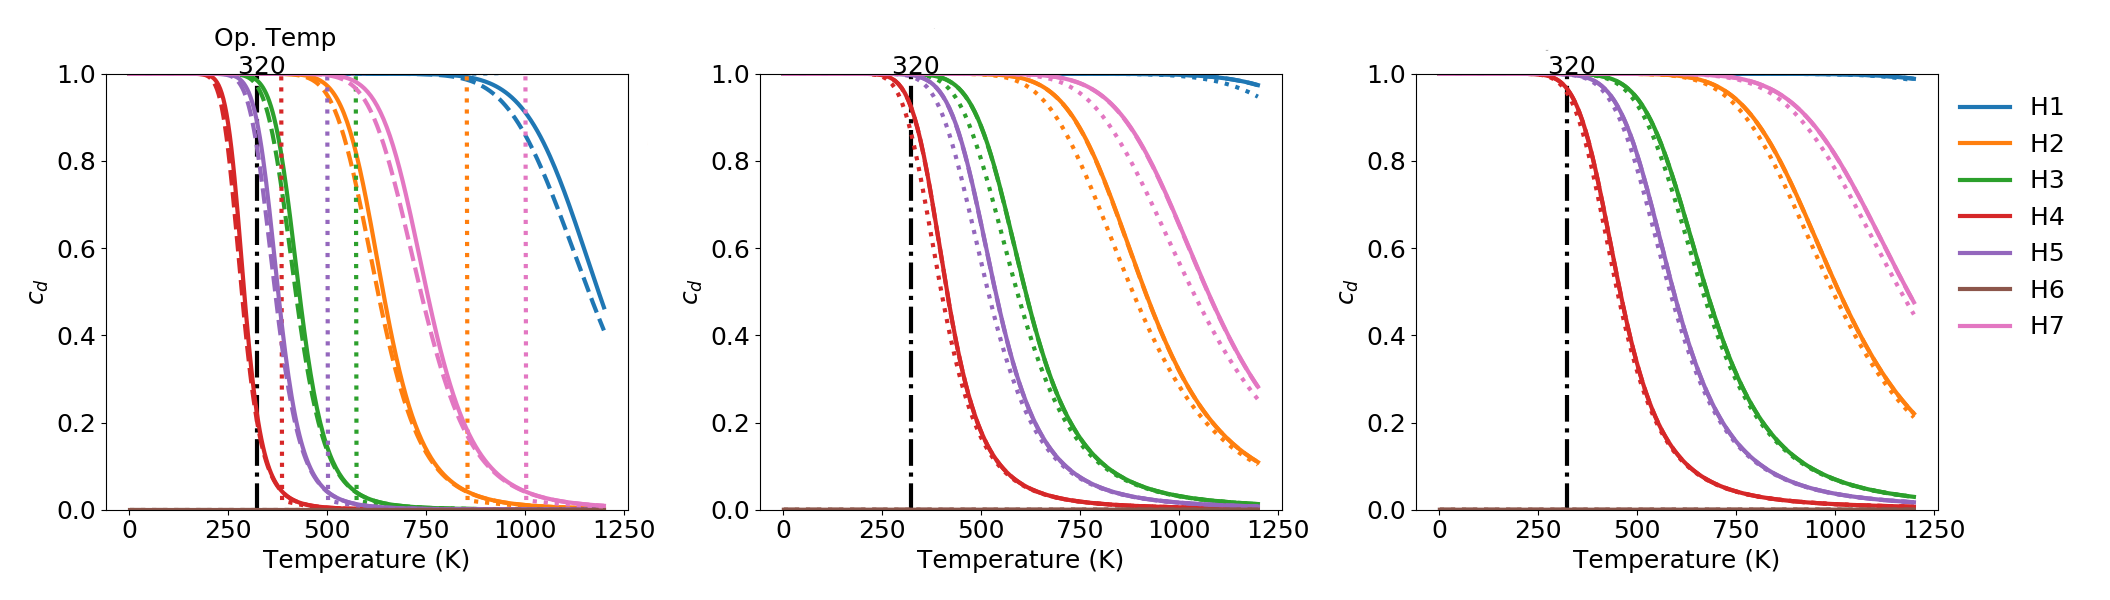
\includegraphics[width=1.65\textwidth]{Images/cd_hard_core_ferrite_sc_all_10_433_1000_appm.png}  \\

          	   \end{tabular}		
   \caption{ Variation of carbon concentration on the dislocation line $c_d$ for each of the binding sites for the easy core (top) and hard core (bottom). Solid, dashed and dotted lined correspond to dislocation densities of $1\times10^{12}$, $1\times10^{14}$ and $5\times10^{15}$ respectively. The nominal carbon concentrations are 10 appm (left) and 1000 appm (right), with the middle figures taken to be the concentration of carbon at the solubility limit C in ferrite: 0.02wt\% $\approx433$ appm. $c_d$ and $c_{\text{bulk}}$ reached self-consistency, with an absolute tolerance of $1\times10^{-3}$. C-C interactions were not taken into account. The concentration of carbon around the easy core, drops off at a lower temperature than that of the hard core due to lower binding energies, with reduction in concentration  The operating temperature is taken to be $50\deg$ C $= 320 \deg$ K. }
   \label{cdhardeasy}
      \end{figure}
      \end{landscape}






\subsection{Progression to Line Tension Model}
\label{sec:orge4b32c9}


The \(K\) coefficient for the line tension model was calculated from atomistic simulations, using
the method of Itakura \cite{Itakura2012}, by calculation of a Hessian from the displacement of
atoms surrounding the dislocation core. Tight-binding gave \(K = 0.734\) eV\AA{}\(^{-2}\), which agrees well
with DFT, where \(K = 0.816\) eV\AA{}\(^{-2}\).


\begin{figure}[htbp]

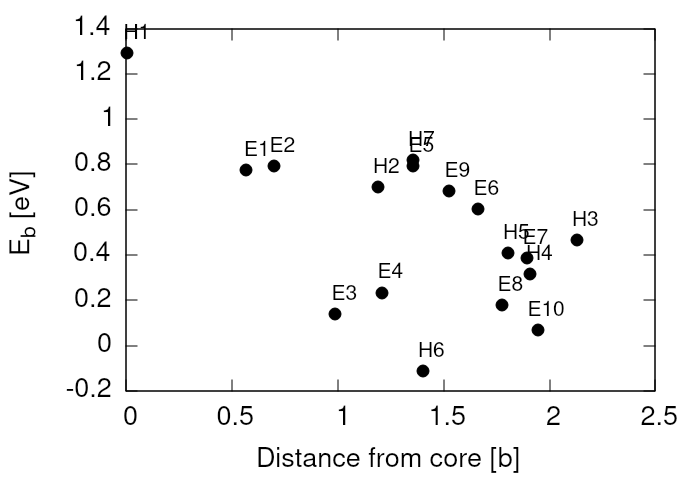
\includegraphics[width=0.8\textwidth]{/home/tigany/Documents/docs/Management/Images/fe_c_binding_energy_distance.png}
\caption{Distance dependence of the binding energies of carbon to the \(1/2\langle 111 \rangle\) screw dislocation in iron. Positive binding energies denote a favourable binding. \label{distancedep}}
\end{figure}

Dislocation-carbon binding energies were found to decay with distance, as seen in figures
\ref{distancedep} and \ref{lorentzianfit}. A Lorentzian was fit to specific binding energies such
that a continuous function could be used to describe binding within
the line tension model. This is a purely empirical model. The
choice of sites used for the fitting is discussed in section \ref{sec:discussion}.




\begin{figure}[htbp]

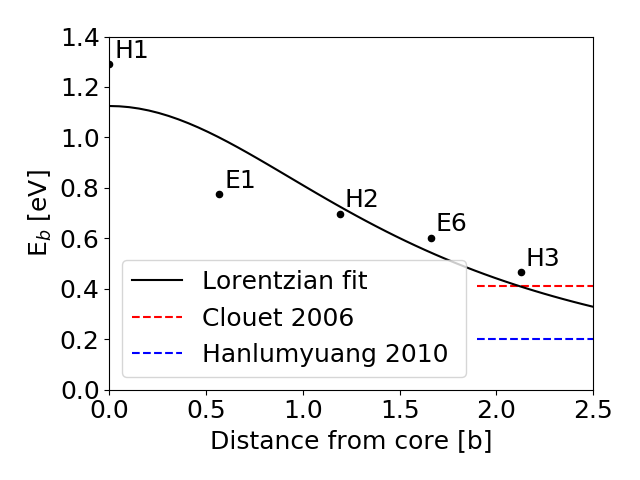
\includegraphics[width=0.8\textwidth]{/home/tigany/Documents/docs/Management/Images/fe-c_lorentzian_fit_binding_energies2.png}
\caption{Fit of Lorentzian to carbon-dislocation binding energies. The sites chosen to fit to were determined by those sites a prismatic carbon in a hard core configuration would find itself, if the dislocation were to move without it along the \(X = \langle\bar{2}11\rangle\) direction. \label{lorentzianfit}}
\end{figure}



\section{Discussion}
\label{sec:org3dae4fb}
\label{sec:discussion}


We expect a reduction in the kink-pair formation enthalpy in tight-binding, due to the
slightly smaller overall Peierls potential along the expected minimum enthalpy path of the
kink. This would increase the rate of kink nucleation in kMC models, causing a higher
overall dislocation velocity. This will increase the disparity between the dislocation velocity and the
speed of carbon diffusion. In the vicinity of the dislocation line, there
is a "high-mobility" zone for carbon to diffuse easily around the dislocation
\cite{Nematollahi2016}. Assuming a similar kink shape as found in EAM calculations, we expect
the kink-pair formation energy to be \(\sim 0.7\) eV, which similar in magnitude to the DFT
value (\(0.73\) eV) \cite{Itakura2012}. Hence, we predict the increase in dislocation velocity
would not so large as to effectively negate the effect of the high-mobility zone---which
would result in carbon not being able to "catch-up" to dislocations upon
movement. Therefore, we do not expect the observed discrepancy in the Peierls potential to
significantly change the principal mechanisms observed, or results obtained, from kMC
simulations of dislocation-assisted carbon migration.



As in Lüthi \cite{Lthi2019}, carbon interactions were found to be vital in understanding how screw
dislocations move in steels, due to the spontaneous reconstruction of the pure iron ground state
(easy core) upon introduction of carbon. From the large binding energy of the H1 site, one would
expect a hard core with carbon in a prismatic site as the ground state configuration for pinned
dislocations.

In the context of dislocation-assisted carbon migration, with sufficient contact stress,
dislocations in their hard core ground state will be forced to move (say, along the \(X =
    \langle\bar{2}11\rangle\) direction), which results in the hard core reconstructing to an easy core. Due to
the much higher velocity of dislocations, relative to the diffusivity of carbon, the
prismatic carbon will stay in-place, becoming an E1 site. A drag force now acts to impede motion of the
dislocation, due to the binding of the carbon in the E1 site. Progression of dislocation glide
results in further reconstruction of the dislocation core to hard and easy states, with the
original carbon being situated in H2, E6 and H3 sites, relative to the dislocation
centre. Thus as the dislocation moves, there is a significant drag force acting on the
dislocation, which decreases the further the dislocation moves from carbon, as one would
expect. This suggests that a dislocation-assisted carbon migration mechanism could be feasible,
but the last two stages of the multi-scale model are necessary to verify this.


In normal operating temperatures of the bearing, one expects all dislocations to be hard cores
saturated with carbon (neglecting C-C interaction) in most of the \(\text{H}j\) sites, as seen in
the concentration analysis. In ferrite that has just transformed, assuming a C concentration of
0.6 wt\% as seen in martensite, we expect similar behaviour to the 1000 appm case as seen in
figure \ref{cdhardeasy}. Including C-C interactions would reduce these concentrations from
saturation. There is insufficient data to say how strong this effect would be.



\section{Future work}
\label{sec:org04ce3e2}

The prerequisites for a line tension model are in place for determination of the kink-pair
formation enthalpies of screw dislocations as a function of carbon content and stress. This is
ongoing work. Validation tests will be carried out on the Itakura data set for the binding of
hydrogen to screw dislocations in bcc iron.


Using the kink-pair formation enthalpies and the binding energies of carbon to screw dislocations, one can proceed
with kinetic Monte Carlo simulation of dislocation glide, in an environment of carbon to
understand how dislocations move carbon under applied stress, in different temperature
and nominal carbon concentration regimes.


It would be of interest to pursue atomistic calculations of carbon bound to edge
dislocations. Recent DFT/Eshelby theory calculations by Maugis \emph{et al.} \cite{Maugis2020}, show
under \emph{compressive} stress, carbon diffusivity is \emph{enhanced}. Pipe diffusion along edge
dislocations could therefore be an important aspect to consider in carbon transport, in addition
to the higher mobility of edge dislocations in bcc iron. As such, edge dislocations could be quite
important within the mechanism of dislocation-assisted carbon migration.

Ising and Monte Carlo models of intersite carbon interactions have been performed using the
results of DFT carbon-dislocation binding energies \cite{Lthi2019}.  These calculations only
considered the hard core, with carbon binding sites of the H1 prismatic site and a H2 site, (which
they name \(P\) and \(O^{(4)}\) respectively). First neighbour C-C interactions were taken
into account, both along the dislocation line and between carbon sites. Using the tight-binding
calculations detailed in this report, we can easily apply and extend this analysis to consider more
binding sites around the hard core, and observe stable carbon distributions around the easy core.

Analysis of carbon diffusion barriers around a dislocation are necessary. In a DFT/EAM
study of carbon-supersaturated ferrite in pearlitic wires, it was found that carbon can diffuse
easily around the dislocation, which is an important consideration in the drag mechanism proposed
\cite{Nematollahi2016}.

\section{Conclusion}
\label{sec:org969c74c}

Dislocation-assisted carbon migration is thought to be a viable mechanism by which martensite
decays to form DER regions---mostly composed of ferrite interspersed in a martensitic
matrix---which enhances failure risk by RCF. There is dispute over where excess carbon from the
martensitic matrix finds itself upon transformation to ferrite, of much lower carbon
solubility. The current leading mechanism suggests carbon segregates to pre-existing carbides, yet
experimental results show in the late stages of DER formation, pre-existing carbides are partially
dissolved in areas of highly localized plasticity, implying segregation of carbon to
dislocations. As such, a thorough investigation of carbon-dislocation interactions is vital to
understanding how DER initially forms and progresses.

Atomistic calculations using tight-binding, the first stage in a multi-scale paradigm to
understand dislocation-assisted carbon migration, found a Peierls potential with characteristics
comparable to both EAM/DFT results. A canonical \(d\text{-band}\) model may better describe this
energy landscape. It is not expected that the discrepancy in the Peierls potential would
significantly change results in kMC simulations.

Carbon distribution around the easy and hard cores were found to differ
significantly, with the largest binding energy being found by carbon being situated in a prismatic
site in the hard core. Carbon within 3\AA{} of the easy core caused reconstruction to the hard core,
with carbon in a prismatic site.

Equilibrium concentrations of carbon around the hard/easy cores at normal operating temperatures
suggest that all dislocations are of hard core type with carbon situated in a H1/prismatic site, with
reconstruction of all easy core dislocations to hard core, resulting in all dislocations being
pinned.

If a dislocation moves under stress from the hard core-prismatic carbon ground state, a large drag
force acts on the dislocation upon movement to adjacent easy and hard positions, assuming the carbon
will stay in place due to its low diffusion coefficient, relative to dislocation velocity. The
carbon-dislocation binding energies decrease with distance, and are in good agreement with
literature. This suggests that a dislocation-assisted carbon migration mechanism is plausible, but
more work needs to be done to confirm if so.

Further work will be done to ascertain diffusion barriers around the dislocation, which have been
shown to be significantly reduced from bulk values due to the presence of dislocations in DFT/EAM
calculations \cite{Nematollahi2016}. This will complete the description of the solute drag mechanism.

Line tension and kMC models will be used to determine how dislocation glide is affected by carbon
and how carbon can move with dislocations. 


\section{Appendix}
\label{sec:org901956f}
\subsection{Regularisation of interaction energy in quadrupolar array}
\label{sec:org6722687}
\label{sec:Ainteractionenergy}


In isotropic elasticity, the elastic energy of a single dislocation dipole in an
infinite lattice is given by


\[ E_{\text{el}}^{\infty} = \frac{\mu b^2}{4\pi} ln \big( \frac{r}{r_{c}} \big)  \]

The contribution from periodic images to the correction is 

\[ E_{\text{img} } = E_{\text{el}} (\mathbf{a}, \mathbf{c}_i , r_c) - E_{\text{el}}^{\infty}
   (\mathbf{a}, r_c),\]

"Ghost" dipoles are introduced to account for the conditional convergence of the sum at \(\pm\alpha
   \mathbf{b}\) and \(\pm \beta\mathbf{b}\), where \(\alpha = \beta = 0.5\). We define \(E_{\text{dg}} (\mathbf{R})\) as the
interaction energy of a ghost dislocation and a dipole at \(\mathbf{R}\) anisotropic elasticity
equations as shown in \cite{Cai2003}.


Defining, 
 \[ E_{\text{dd}} (\mathbf{R}) = \frac{\mu b^2}{2\pi}
   \text{ln}\frac{|\mathbf{R}|^2}{|\mathbf{R}+\mathbf{a}|\cdot|\mathbf{R}-\mathbf{a}|},
   \]
we obtain,
\[ E_{\text{img}} = \frac{1}{2}\sum_{\mathbf{R}} [ E_{\text{dd}} (\mathbf{R}) - E_{\text{dg}} (\mathbf{R}) ] - \frac{1}{2}_{}
   E_{\text{dg}} (\mathbf{R} = 0),  \]

which can be subtracted from the total energy as given from atomistic calculations, for a
regularised interaction energy. 


\subsection{Zero-point energy calculation}
\label{sec:org33492d2}
\label{sec:zeropointenergy}

After relaxation of the C-dislocation system, a 3x3 Hessian matrix is constructed by taking the
numerical derivative of forces observed on the carbon atom after displacement by \(\pm 0.015 \AA\) in
each of the \(X\), \(Y\) and \(Z\) directions.  The three atoms surrounding the core on the first and
third layers were again fixed in \(Z\) coordinate. The zero-point energy is given by

\[ E_z = \frac{1}{2} \sum_{i=1}^3 \frac{h}{2\pi} \sqrt{ k_i /
   m_{\text{C}} },  \]
where \(k_i\) are the eigenvalues of the Hessian and \(m_\text{C}\) is
the mass of carbon. 


\section{Bibliography}
\label{sec:orgeb1b461}
\label{org96a1395}

\bibliographystyle{unsrt}

\bibliography{bibliography/org-refs}
\end{document}